% 2007 年陕西卷文科第 16 题：向量 OA、OB、OC 的夹角关系。
%   OA 与 OB 成 120°，OA 与 OC 成 30°，|OA|=|OB|=1，|OC|=2√3。
% 来源 PDF：gaokaomath-src/普通高考/2007/2007陕西文.pdf
% SHA-256：95abaa3050f33e9b9587ad186af8f173fbf40c31ebe3f2be710bbae607ed0ecb
% 原页：2007陕西文.pdf 第 1 页（A3 三栏）第 3 栏，书页码 403。
% 重绘依据：按原页三个向量的方向与长度比例重绘。
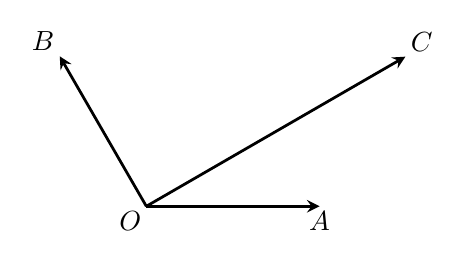
\begin{tikzpicture}[scale=1.0, semithick,
  every node/.style={inner sep=1.5pt}]
  \coordinate (O) at (0,0);
  \coordinate (A) at (2.2,0);
  \coordinate (B) at (-1.1,1.905);
  \coordinate (C) at (3.29,1.9);

  \draw[->,>=stealth,line width=1pt] (O) -- (A) node[below] {$A$};
  \draw[->,>=stealth,line width=1pt] (O) -- (B) node[above left] {$B$};
  \draw[->,>=stealth,line width=1pt] (O) -- (C) node[above right] {$C$};
  \node[below left] at (O) {$O$};
\end{tikzpicture}
